% arara: lualatex: { synctex: on, shell: off }
% arara: biber
% arara: lualatex: { synctex: on, shell: off }
% arara: sumatrapdf
\documentclass[../main.tex]{subfiles}

% %Set the package to import preambles
\usepackage{subfiles}

%Load graphicx here to specify options
\usepackage[final]{graphicx}

%Set the document font
\usepackage[no-math]{fontspec}
\setmainfont[Ligatures=TeX]{Times New Roman}
\setmonofont{Inconsolata}

%Set the text to double spacing
%According to hyperref README,
%setspace should be loaded first
\usepackage[doublespacing]{setspace}

%Set a command to easily skip a line
\newcommand{\blankline}{\vspace*{\baselineskip}}

%Set up biblatex
\usepackage[
    backend=biber,
    % url=false,
    doi=true,
    sorting=none,
    sortcites=true,
    maxbibnames=6,
    minbibnames=6,
    maxcitenames=2,
    mincitenames=1,
    citestyle=numeric-comp,
    firstinits=true,
    isbn=false
]{biblatex}
\addbibresource{C:/Users/\user/Documents/Github/dissertation/library.bib}

%Remove the "In:" from before the journal title for articles
\renewbibmacro{in:}{%
  \ifentrytype{article}{}{\printtext{\bibstring{in}\intitlepunct}}}

%Change the name of the bibliography section to "References"
\DefineBibliographyStrings{english}{bibliography = {References}}

%Set the sort order of the names in each bibliography entry
\DeclareNameAlias{default}{last-first}

%Don't print the article title. To print the title, add #1 to the last {}
\DeclareFieldFormat[article,incollection,unpublished]{title}{}

%Add "vol." and "no." before volume and issue.
\DeclareFieldFormat[article]{volume}{\bibstring{volume}\addspace #1}
\DeclareFieldFormat[article]{number}{\bibstring{number}\addspace #1}

%Ensure that a comma follows abbreviated journal titles.
\DeclareFieldFormat{journaltitle}{\mkbibemph{#1}\isdot}

%Put a comma between the volume and issue instead of period.
\renewbibmacro*{volume+number+eid}{%
  \printfield{volume}%
  \setunit{\addcomma\space}%<---- was \setunit*{\adddot}%
  \printfield{number}%
  \setunit{\addcomma\space}%
  \printfield{eid}}

%Add a comma after the journal title.
\renewbibmacro*{journal+issuetitle}{%
  \usebibmacro{journal}%
  \setunit*{\addcomma\addspace}%<---- was \setunit*{\addspace}%
  \iffieldundef{series}
    {}
    {\newunit
     \printfield{series}%
     \setunit{\addspace}}%
  \usebibmacro{volume+number+eid}%
  \setunit{\addspace}%
  \usebibmacro{issue+date}%
  \setunit{\addcolon\space}%
  \usebibmacro{issue}%
  \newunit}

%Only print URL if doi is not present.
\DeclareFieldFormat{url}{%
  \iffieldundef{doi}{%
    \mkbibacro{URL}\addcolon\space\url{#1}%
  }{%
  }%
}
\DeclareFieldFormat{urldate}{%
  \iffieldundef{doi}{%
    \mkbibparens{\bibstring{urlseen}\space#1}%
  }{%
  }%
}

%Remove publisher from being printed.
\renewbibmacro*{publisher+location+date}{%
  \printlist{location}%
  \setunit*{\addcomma\space}%
  \usebibmacro{date}%
  \newunit}

%Fix in-text full citations
\DeclareCiteCommand{\fullcite}
  {\usebibmacro{prenote}}
  {\usedriver
     {\defcounter{minnames}{99}%
      \defcounter{maxnames}{99}}
     {\thefield{entrytype}}}
  {\multicitedelim}
  {\usebibmacro{postnote}}

%Use fancy tables.
\usepackage{booktabs}

%Set up todo notes in the PDF file
\usepackage{todonotes}

%Use and set up the caption package for nicer captions.
\usepackage{caption}
\DeclareCaptionLabelFormat{bf}{\textbf{#1 #2}}
\captionsetup{
    font=small ,
    labelsep=colon ,
    labelformat=bf ,
    figurewithin=chapter ,
    tablewithin=chapter ,
}

\usepackage{titlesec}
\usepackage{titletoc}

\titleformat{\chapter}[display]{\normalfont\Huge\bfseries}{Chapter \thechapter}{0.7em}{}
\titleformat{\section}{\normalfont\LARGE\bfseries}{\thesection}{0.5em}{}
\titleformat{\subsection}{\normalfont\Large\bfseries}{\thesubsection}{1em}{}
\titleformat{\subsubsection}{\normalfont\large\bfseries}{\thesubsubsection}{1em}{}

\titlecontents{chapter}[0pc]{}{\bfseries Chapter \thecontentslabel\quad}{}{\titlerule*[0.5pc]{.}\contentspage}
\titlecontents{section}[1em]{}{\thecontentslabel\quad}{}{\titlerule*[0.5pc]{.}\contentspage}
\titlecontents{subsection}[2em]{}{\thecontentslabel\quad}{}{\titlerule*[0.5pc]{.}\contentspage}
\titlecontents{subsubsection}[3em]{}{\thecontentslabel\quad}{}{\titlerule*[0.5pc]{.}\contentspage}

\setcounter{secnumdepth}{3}
\setcounter{tocdepth}{3}

%Use the subfigure package
\usepackage{subfig}

%Various math improvements.
%Must be loaded before hyperref
\usepackage{mathtools}

%Set the math font. Has to come after mathtools because
%some font stuff gets overwritten.
\usepackage{unicode-math}
\unimathsetup{math-style=TeX}
\setmathfont[range=\mathup/{num}]{Times New Roman}
\setmathfont[range=\mathit/{greek,Greek,latin,Latin}]{Cambria Math}
\setmathfont[range=\mathup/{greek,Greek,latin,Latin}]{Cambria Math}
\setmathfont[range={"2212,"002B,"003D,"0028,"0029,"005B,"005D,"221A,
"2211,"2248,"222B,"007C,"2026,"2202,"00D7,"0302,"2261,"0025,"22C5,
"00B1,"2194,"21D4,"2260}]
{Cambria Math}

%Better looking fonts
\usepackage[final]{microtype}

%Allow table cells to span multiple rows.
\usepackage{multirow}

%Allow landscape rotated figures and captions.
\usepackage{afterpage}
\usepackage{rotating}
\usepackage{pdflscape}

%Set the root path where figures are stored.
\graphicspath{ {C:/Users/\user/Documents/Github/dissertation/figures/} }

%Set a convenience command for table cells that allow line breaks.
\newcommand{\linebreakcell}[2][c]{%
  \begin{tabular}[#1]{@{}c@{}}#2\end{tabular}}

%Use and set up the siunitx package for nice units printing.
\usepackage{siunitx}
\sisetup{%
    group-separator = {,},
    range-phrase = {\text{ to }},
    list-separator = {\text{, }},
    list-final-separator = {\text{, and }},
    list-pair-separator = {\text{ and }},
}%
\DeclareSIUnit\calorie{cal}
\DeclareSIUnit\atmosphere{atm}
\DeclareSIUnit\torr{torr}

%Declare convenience macros for printing the
%names of the alcohols.
\newcommand{\iPeOH}{\textit{i}-pentanol}
\newcommand{\nBuOH}{\textit{n}-butanol}
\newcommand{\sBuOH}{\textit{s}-butanol}
\newcommand{\tBuOH}{\textit{t}-butanol}
\newcommand{\iBuOH}{\textit{i}-butanol}

%The floatrow package allows multiple floats in a row
%and is set so that table captions are on top of the
%table.
\usepackage{floatrow}
\floatsetup[table]{style=plaintop}

%Use the titling package to allow easy access to custom title pages
\usepackage{titling}
\title{High Pressure Ignition Chemistry of Alternative Fuels}
\author{Bryan William Weber}

%Add bibliography and indices to the TOC
\usepackage{tocbibind}

%Improve handling of appendices
\usepackage{appendix}

%Use package that allows inline patching of commands. This is used in
%the appendices section.
\usepackage{xpatch}

%Use the bookmark package (which loads hyperref) so that only one
%compilation is necessary to get references.
\usepackage{bookmark}

%Set the color of the links and PDF metadata
\hypersetup{%
    pdfinfo={
        Title={High Pressure Ignition Chemistry of Alternative Fuels},
        Author={Bryan W. Weber},
    },
    colorlinks=true,
    citecolor=blue,
    linkcolor=black,
    plainpages=false,
    final,
}

%Allow lualatex to properly add links processed from pax files.
\usepackage{pdftexcmds}
\makeatletter
\let\pdfescapename=\pdf@escapename
\let\pdfstrcmp=\pdf@strcmp
\makeatother
\usepackage{pax}

%Allow to use \doi to link to DOI links.
\usepackage{doi}

%Allow inserting PDF documents directly to the output. According to
%http://tex.stackexchange.com/a/13660/32374, should come after hyperref
\usepackage{pdfpages}

%Do a better job with the automatic references. According to
%http://tex.stackexchange.com/a/1868/32374, should come after hyperref
\usepackage[capitalise, sort&compress]{cleveref}

%Set the auto-format names for the cleveref operations
\crefname{chapter}{Chapter}{Chapters}
\Crefname{chapter}{Chapter}{Chapters}
\crefname{section}{Sec.}{Secs.}
\Crefname{section}{Section}{Sections}
\crefname{subsection}{Sec.}{Secs.}
\Crefname{subsection}{Section}{Sections}
\crefname{subsubsection}{Sec.}{Secs.}
\Crefname{subsubsection}{Section}{Sections}
\crefname{figure}{Fig.}{Figs.}
\Crefname{figure}{Figure}{Figures}
\crefname{table}{Table}{Tables}
\Crefname{table}{Table}{Tables}
\crefname{equation}{Eq.}{Eqs.}
\Crefname{equation}{Equation}{Equations}
\crefname{appchap}{Appendix}{Appendices}
\Crefname{appchap}{Appendix}{Appendices}

\newcommand{\creflastconjunction}{, and~}
\newcommand{\crefrangeconjunction}{--}

%Set the size of the margins and the paper
%According to http://tex.stackexchange.com/a/26592/32374
%this should go after hyperref
\usepackage[margin=1in, letterpaper]{geometry}

%Set up the page numbers
%This has to go after geometry so the page number is centered
\usepackage{fancyhdr}
\pagestyle{fancy}
\fancyhf{}
\fancyfoot[C]{\thepage}
\renewcommand{\headrulewidth}{0pt}


\begin{document}

\begin{figure}[!ht]\CenterFloatBoxes
    \begin{floatrow}
        \killfloatstyle\ttabbox
        {\captionsetup{type=table}\caption{HHV of Ethanol, \textit{i}-Pentanol, and Gasoline}
        \label{tab:ipeoh-heats}}
        {\begin{tabular}{*{4}{c}}
            \toprule
            Compound & Ethanol \cite{Afeefy2014} & \textit{i}-Pentanol \cite{Afeefy2014} & Gasoline \cite{Davis2013} \\
            \midrule
            HHV [\si[per-mode=symbol]{\mega\joule\per\kilo\gram}] & 29.67 & 37.73 & 48.46 \\
            \bottomrule
        \end{tabular}}
        \ffigbox[\FBwidth]
            {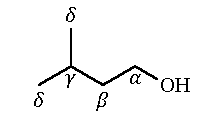
\includegraphics[width=5cm]{04-Pentanol/ipeoh-skeletal}}
            {\caption{Skeletal structure of \iPeOH{}}
            \label{fig:ipeoh-skeletal}}
    \end{floatrow}
\end{figure}

\section{Structure of \textit{i}-Pentanol}
\label{sec:ipeoh-struct}

\textit{i}-Pentanol (3-methyl-1-butanol) is a five-carbon alcohol whose
skeletal structure is shown in \cref{fig:ipeoh-skeletal}. The carbon
atoms in \cref{fig:ipeoh-skeletal} are labeled according to their
distance from the hydroxyl moeity, with $\alpha$ being the closest and
$\delta$ being the farthest. The Greek letter notation will be used to
refer to the carbon-centered radicals in \cref{sec:ipeoh-discussion}.
\textit{i}-Pentanol can be produced biologically \cite{Peralta-Yahya2012},
and offers several similar advantages as the butanol isomers compared
to ethanol. \Cref{tab:ipeoh-heats} compares the HHV of ethanol, \iPeOH{},
and gasoline.

\section{Procedures}
\label{sec:ipeoh-procedure}

Experiments for \iPeOH{} in the RCM have been performed at the conditions listed
in \cref{tab:ipeoh-expts}. Homogeneous fuel and air pre-mixtures are prepared in an approximately
\SI{17}{\liter} mixing tank. The mixing tank and all tubes and manifolds
connecting the tank with the RCM are heated, allowing the study of
relatively low vapor pressure fuels. The initial temperature is set above
the saturation temperature of \iPeOH{} for each mixture studied. The mixing
tank is equipped with a magnetic stirrer to ensure complete homogeneity
of the mixture.

\begin{table}
    \caption{\iPeOH{} Experimental Conditions}
    \label{tab:ipeoh-expts}
    \begin{tabular}{*{5}{c}}
    \toprule
    \multicolumn{3}{c}{Reactant (Purity)} & \multirow{3}[0]{*}{\linebreakcell{Equivalence \\ Ratio \\ $\phi$}} & \multirow{3}[0]{*}{\linebreakcell{Compressed \\ Pressure \\ $P_C$ (bar)}} \\
    \cmidrule{1-3}
    \linebreakcell{\iPeOH{} \\ (\SI{99.6}{\percent})} & \linebreakcell{O$_2$ \\ (\SI{99.994}{\percent})} & \linebreakcell{N$_2$ \\ (\SI{99.999}{\percent})} & & \\
    \cmidrule{1-3}
    \multicolumn{3}{c}{Mole Percentage}   & & \\
    \midrule
    2.41 & 20.50 & 77.09 & 1.0 & 40 \\
    1.22 & 20.75 & 78.03 & 0.5 & 40 \\
    4.71 & 20.01 & 75.27 & 2.0 & 40 \\
    \bottomrule
    \end{tabular}
\end{table}

Prior to mixture preparation, the mixing tank is vacuumed to less than
\SI{1}{\torr}, whereupon liquid fuel (\iPeOH{}, Sigma-Aldrich, \SI{99.6}{\percent}
purity) is injected by a syringe through a septum. The syringe is massed
before and after the injection, with the difference being the amount of
fuel in the mixing tank. Based on this mass, required proportions of
the gaseous oxidizer (O2, \SI{99.994}{\percent} purity, N2, \SI{99.999}{\percent} purity) are
calculated. The gases are added to the mixing tank sequentially at
room temperature and the total pressure is monitored to ensure that the
proper mixture concentrations are attained. Finally, the heaters and
stirring vane are switched on and the system is allowed approximately
\SI{1.5}{\hour} to reach steady state.

\section{Model Improvements}
Through collaboration with researchers at Lawrence Livermore National
Laboratory, many improvements to the chemical kinetic model for \iPeOH{} were
made relative to the work of \textcite{Tsujimura2012}. Some of the major
improvements are highlighted below; see the article for more detail
\cite{Sarathy2013}.

\begin{enumerate}
\item The model was restructured based on work with C$_4$ and C$_5$
      alcohols \cite{Sarathy2012, Heufer2012a}
\item The most stable conformers of \iPeOH{} were calculated using
      quantum chemistry software
\item The BDEs of the of the C-C, C-H, C-O, and O-H bonds were calculated
      using quantum chemistry software
\item The model includes the Waddington pathway shown to be important in
      low-temperature decomposition of \iPeOH{} by \textcite{Welz2012}
\item New reaction pathways were added based on the work of \textcite{Welz2012,
      Welz2013}, including the unconventional water-elimination pathway discussed
      in \textcite{Welz2013}
\end{enumerate}

Moreover, the following data sets from the literature and presented in
the work of \textcite{Sarathy2013} were used to validate the newly
updated model, in addition to the new data at $P_C=\SI{40}{\bar}$ presented here.

\begin{enumerate}
\item Ignition delays measured in a ST and an RCM\cite{Tang2013, Tsujimura2012}
\item JSR species data \cite{Dayma2011}
\item New ignition delays measured in STs \cite{Sarathy2013}
\item New JSR species data \cite{Sarathy2013}
\item New flame speed and flame extinction measurements \cite{Sarathy2013}
\end{enumerate}

\section{Experimental \& Modeling Results}
\label{sec:ipeoh-results}

The experimental ignition delays measured in the RCM are shown in
\cref{fig:ipeoh-7bar,fig:ipeoh-20bar,,fig:ipeoh-40bar}, along with
ignition delays measured in the ST and comparison with
the model simulations. There is no $\phi=2.0$ data set for \SI{7}{\atmosphere}
because no conditions at which ignition occurred could be found.
In \cref{fig:ipeoh-7bar,fig:ipeoh-20bar,fig:ipeoh-40bar}, solid
lines represent adiabatic, constant volume simulations, and dashed
lines represent volume-profile simulations.

\begin{figure}
    \ffigbox[\FBwidth]
        {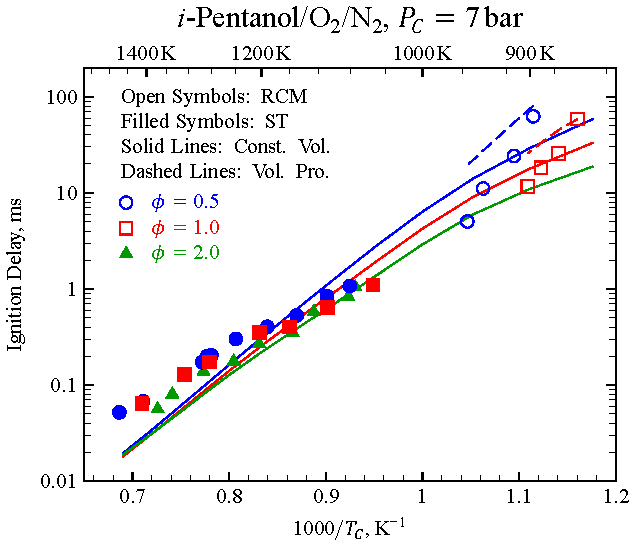
\includegraphics[width=10cm]{04-Pentanol/ipeoh-7bar}}
        {\caption{ST and RCM ignition delay times from
        \textcite{Tsujimura2012} at \SI{7}{\atmosphere} compared
        with model predictions by the model from \textcite{Sarathy2013}.}
        \label{fig:ipeoh-7bar}}
    \par
    \vspace{10pt}
    \ffigbox[\FBwidth]
        {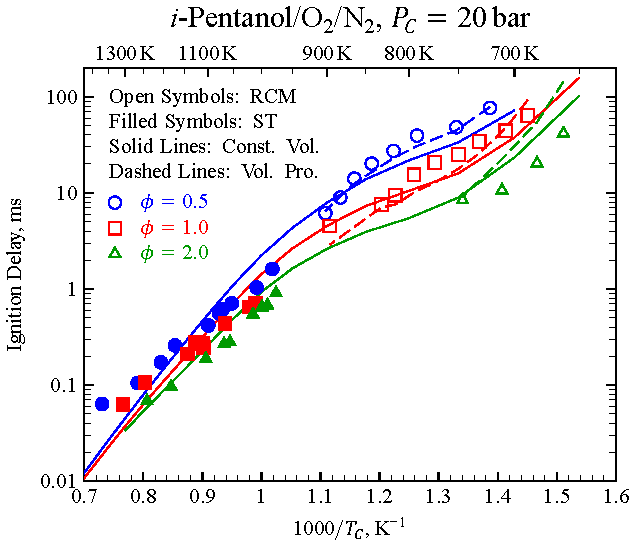
\includegraphics[width=10cm]{04-Pentanol/ipeoh-20bar}}
        {\caption{ST and RCM ignition delay times from
        \textcite{Tsujimura2012} at \SI{20}{\atmosphere} compared
        with model predictions by the model from \textcite{Sarathy2013}.}
        \label{fig:ipeoh-20bar}}
\end{figure}
\begin{figure}
    \ffigbox[\FBwidth]
        {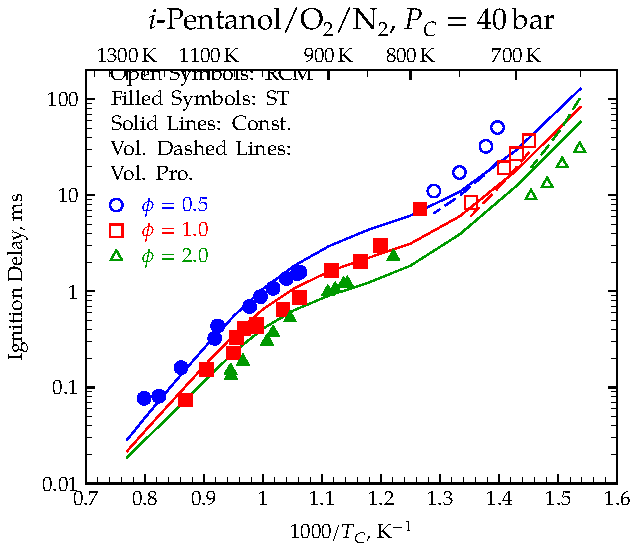
\includegraphics[width=10cm]{04-Pentanol/ipeoh-40bar}}
        {\caption{ST and RCM ignition delay times from
        \textcite{Sarathy2013} at \SI{40}{\atmosphere} compared
        with model predictions by the model from \textcite{Sarathy2013}.}
        \label{fig:ipeoh-40bar}}
    \par
    \vspace{10pt}
    \ffigbox[\FBwidth]
        {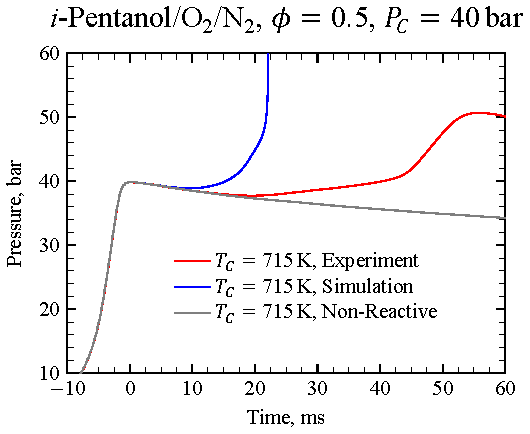
\includegraphics[width=10cm]{04-Pentanol/ipeoh-phi05}}
        {\caption{Experimental reactive (red), simulated reactive
        (blue), and experimental non-reactive (gray) pressure
        profiles at \SI{40}{\atmosphere} for lean \iPeOH{}/air mixtures.}
        \label{fig:ipeoh-phi05}}
\end{figure}
\begin{figure}
    \ffigbox[\FBwidth]
        {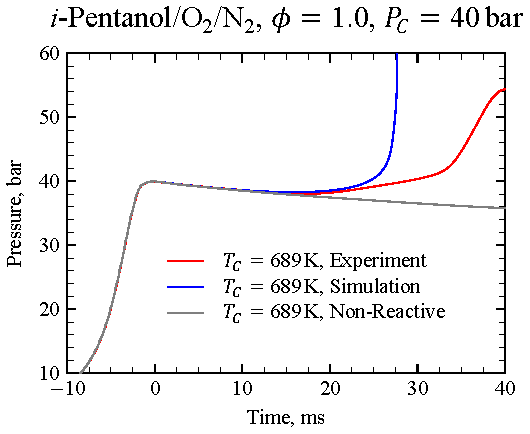
\includegraphics[width=10cm]{04-Pentanol/ipeoh-phi10}}
        {\caption{Experimental reactive (red), simulated reactive
        (blue), and experimental non-reactive (gray) pressure
        profiles at \SI{40}{\atmosphere} for stoichiometric \iPeOH{}/air mixtures.}
        \label{fig:ipeoh-phi10}}
    \par
    \vspace{10pt}
    \ffigbox[\FBwidth]
        {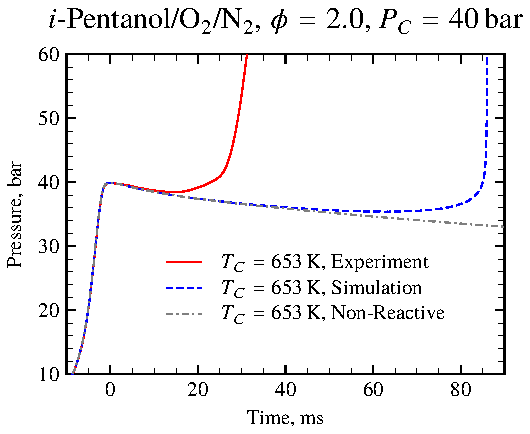
\includegraphics[width=10cm]{04-Pentanol/ipeoh-phi20}}
        {\caption{Experimental reactive (red), simulated reactive
        (blue), and experimental non-reactive (gray) pressure
        profiles at \SI{40}{\atmosphere} for rich \iPeOH{}/air mixtures.}
        \label{fig:ipeoh-phi20}}
\end{figure}

At \SI{7}{\atmosphere} (\cref{fig:ipeoh-7bar}), the high-temperature ignition delays
measured in the ST are generally predicted to within a factor of 1.5. The RCM experiments
are also well predicted at low temperature---within a factor of 2---but
the disagreement grows to approximately a factor of 4 in the
intermediate temperature regime. At \SI{20}{\atmosphere} (\cref{fig:ipeoh-20bar}), the
high-temperature ignition delays are well predicted, including
capturing the equivalence ratio sensitivity of the ignition delays.
The ignition delays measured in the RCM are fairly well predicted
at the lean and stoichiometric conditions, but are over-predicted
at the rich condition.

At \SI{40}{\atmosphere} (\cref{fig:ipeoh-40bar}), the model is able to
reproduce the high-temperature ignition delays fairly well, including
capturing the equivalence ratio dependence of the ignition delays.
Ignition delay data near \SI{40}{\atmosphere} and temperatures
ranging from \SIrange{651}{776}{\kelvin} were also acquired using the
RCM. The ignition data in the RCM and ST are in good qualitative
agreement, displaying the expected decrease in ignition delay with
increasing temperature. The model well predicts the observed trend
of decreasing ignition delay time with increasing equivalence
ratio, which occurs because a higher fuel concentration results
in greater radical production at these conditions. Constant volume
and volume history simulations at the \SI{40}{\atmosphere} RCM
conditions (\cref{fig:ipeoh-40bar}) indicate the model can well predict
ignition delay times at stoichiometric conditions, but cannot well predict
RCM ignition delay data at lean and rich conditions. The difference
(i.e., spread) in ignition delay times across various equivalence ratios
is similar to that observed for other alcohols in the same facilities
(e.g., \nBuOH{} at \SI{15}{\bar} \cite{Weber2011} and \tBuOH{} at
\SI{30}{\bar} \cite{Weber2013}). The primary issue with the model is
its equivalence ratio sensitivity; predicted ignition delay times need
to be increased at lean conditions yet decreased at rich conditions,
implying that the system’s reactivity is controlled by different phenomenon
at different equivalence ratios. At these low temperatures the model’s
reactivity is driven by the overall peroxy reaction sequence,
R+O$_2$=ROO=QOOH(+O$_2$)=OOQOOH=2OH+products, including the inhibitive
direct (i.e., concerted) HO$_2$ elimination and QOOH decomposition routes.
An increase (or decrease) in any reaction rate constant along this
reaction sequence will move the reactivity of the system in the same
direction at all equivalence ratios. Therefore, we were unable to
identify a single reaction rate constant modification that would decrease
overall reactivity at lean conditions while increase it at rich conditions.

Representative experimental and simulated pressure profiles for the lean,
stoichiometric, and rich conditions are shown in
\cref{fig:ipeoh-phi05,fig:ipeoh-phi10,,fig:ipeoh-phi20} respectively,
with the profiles shifted so EOC occurs at \SI{0}{\second}. Interestingly,
the experimental pressure traces after the induction period do not show
a sharp increase in pressure (i.e., heat release is more gradual,
similar to two-stage ignition). For the lean case, there is a moderate
heat release \SI{25}{\milli\second} after EOC followed by a larger heat
release event, and similar behavior is observed at other equivalence ratios.
It is noted that similar heat release prior to the main ignition event
was found in an HCCI engine experiment using \iPeOH{} by \textcite{Yang2010}
and was termed Intermediate Temperature Heat Release (ITHR) in their
work.

The pressure profile of the present simulations qualitatively
agrees with the experimental data, in that the simulated pressure
traces deviate from the non-reactive trace prior to the main ignition
event, although the ignition delay itself does not necessarily
agree very well. For lean and stoichiometric cases the simulated
ignition delay times are fast compared to the data, whereas at rich
conditions they are too slow.

\section{Discussion}
\label{sec:ipeoh-discussion}

The sensitivity of the ignition delay to changes in the reaction rate
coefficients is shown in \cref{fig:ipeoh-20sens} for a constant volume,
adiabatic simulation at \SI{20}{\atmosphere}, \SI{800}{\kelvin}, and for
equivalence ratios varying from $\phi=\numrange{0.5}{2.0}$. The percent
sensitivity is computed by the formula:
%
\begin{align}
S = \frac{\tau(2k_i)-\tau(k_i)}{\tau(k_i)} \times \SI{100}{\percent}
\end{align}
%
where $\tau(2k_i)$ is the ignition delay when the rate coefficient of
reaction $i$ is doubled, and $\tau(k_i)$ is the nominal ignition delay.
Positive sensitivities therefore represent an increase in the ignition
delay when the rate coefficient of reaction $i$ is increased. Both the
forward and reverse rates of each reaction are increased simultaneously.
Since the reaction 2ho2$\Leftrightarrow$h2o2+o2 is represented by two sets of $\mathrm{A}$, $b$,
and $E_a$ in the reaction mechanism, both Arrhenius coefficients were
simultaneously doubled to give the sensitivity value shown in \cref{fig:ipeoh-20sens}.

It is seen from \cref{fig:ipeoh-20sens} that the most sensitive reaction
under these conditions is H-abstraction by OH to form the $\alpha$-hydroxypentyl
radical (ic5h10oh-1). Increasing the rate of abstraction by OH from the
$\alpha$ site increases the ignition delay because subsequent reaction
of the fuel radical with O$_2$ leads to the formation of HO$_2$ and
\textit{i}-pentanal, which is an OH terminating pathway. The next most
sensitive reaction is H-abstraction by OH to form the $\gamma$-hydroxypentyl
radical (ic5h10oh-3). The ignition delay is also sensitive to the rates of
isomerization of the ROO radicals formed by the other hydroxypentyl
radicals. This indicates that, except for the $\alpha$ radical, the
other hydroxypentyl radicals undergo typical low-temperature chain branching
reactions. This observation is further corroborated by a reaction path
analysis, discussed below. Furthermore, \cref{fig:ipeoh-20sens} shows that
the ignition delay is also sensitive to some low temperature chain
terminating pathways, such as formation of an enol + HO$_2$ from ROO
or QOOH radicals.

A sensitivity analysis of the ignition delay to changes in the
reaction rate coefficients for initial conditions of \SI{40}{\atmosphere}
and \SI{689}{\kelvin}, for three equivalence ratios, is shown in
\cref{fig:ipeoh-40sens}. As before, positive sensitivity indicates
that increasing the rate coefficient of that reaction increases the
ignition delay. Similar to the \SI{20}{\atmosphere} sensitivity analysis,
the most sensitive reactions are the H-abstractions from the fuel and
the subsequent reactions of these initial fuel radicals. However,
stronger equivalence ratio dependence of the sensitivity results is
seen in \cref{fig:ipeoh-40sens} compared to \cref{fig:ipeoh-20sens}.
It is interesting to note that the most sensitive reaction, formation
of the $\alpha$-hydroxypentyl radical through H-abstraction by
OH, is nearly twice as sensitive at $\phi=0.5$ than at $\phi=2.0$, while
most of the other reactions have nearly the same sensitivity for
the three equivalence ratios.

In addition, the reaction of formaldehyde and hydroxyl radical to form
formyl radical and water is somewhat sensitive, especially for
the lean case. The importance of this reaction is demonstrated by the
path analysis shown in \cref{fig:ipeoh-20path} (similar results are
obtained for a path analysis at \SI{40}{\atmosphere} as at
\SI{20}{\atmosphere}). Formaldehyde is a significant product in
the decomposition of the $\beta$- and $\gamma$-hydroxypentyl radicals,
as well as the pentoxy radical. Furthermore, the reaction of two
hydroperoxyl molecules to form hydrogen peroxide and oxygen molecule is the
seventh most sensitive reaction. This reaction is important as it releases
the most heat during the ITHR period prior to the main ignition for all
three equivalence ratios and because the rapid reaction of the
$\alpha$-hydroxypentyl radical to form \textit{i}-pentanal and hydroperoxyl
is important in alcohol combustion. In view of the equivalence ratio
dependence shown in \cref{fig:ipeoh-40sens}, these sensitivity analysis
results suggest that it may be possible to adjust multiple reaction
rates in the low temperature chain branching pathways to decrease
reactivity at lean conditions but increase reactivity at rich
conditions, which warrants further investigation.

\begin{figure}
    \ffigbox
        {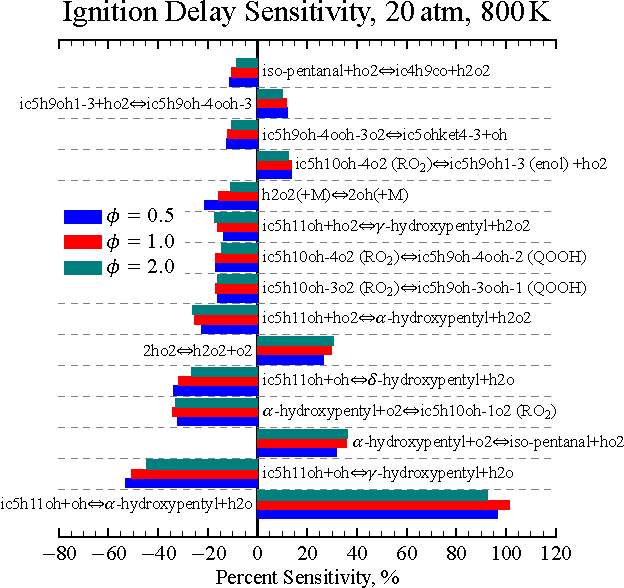
\includegraphics[width=10cm]{04-Pentanol/ipeoh-20sens}}
        {\caption{Sensitivity of the ignition delay to changes in
        the reaction rate coefficients for three equivalence ratios.
        Initial conditions for constant-volume adiabatic simulations are
        \SI{800}{\kelvin} and \SI{20}{\atmosphere}.}
        \label{fig:ipeoh-20sens}}
    \par
    \vspace{10pt}
    \ffigbox
        {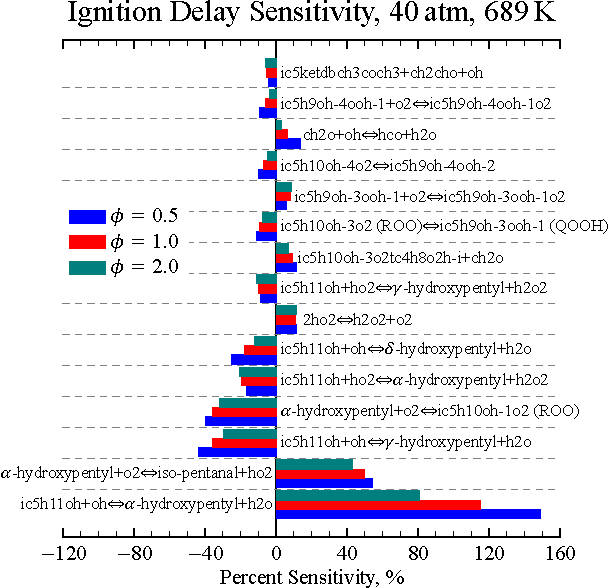
\includegraphics[width=10cm]{04-Pentanol/ipeoh-40sens}}
        {\caption{Sensitivity of the ignition delay to changes in
        the reaction rate coefficients for three equivalence ratios.
        Initial conditions for constant-volume adiabatic simulations are
        \SI{689}{\kelvin} and \SI{40}{\atmosphere}.}
        \label{fig:ipeoh-40sens}}
\end{figure}

The main \iPeOH{} reaction pathways after \SI{20}{\percent} fuel consumption at
\SI{800}{\kelvin}, \SI{20}{\atmosphere}, and for three equivalence
ratios are shown in \cref{fig:ipeoh-20path}, describing the key low
temperature reaction pathways. The percent flux of each reaction path
is the contribution of that path to destroying the reactant, integrated
up to \SI{20}{\percent} fuel consumption. The fuel is mainly consumed by
the H atom abstraction at the $\alpha$ site because \iPeOH{} has a weak
C-H bond at the $\alpha$ site. As discussed previously, subsequent
reactions of $\alpha$-hydroxypentyl with O$_2$ generate \textit{i}-pentanal
+ HO$_2$, an OH terminating pathway. The other hydroxypentyl radicals tend
to add to molecular oxygen and form hydroxyalkylperoxy (ROO) radicals.
These radicals are mainly isomerized to hydroxyalkylhydroperoxide (QOOH)
or decomposed to enol species by the concerted elimination of HO$_2$. Approximately
\SI{18}{\percent} of $\beta$-hydroxyalkylperoxy radicals are decomposed to produce
\textit{i}-butanal (2-methylpropanal), formaldehyde, and OH radical via ROO
isomerization and $\beta$-scission reactions by the Waddington mechanism
\cite{Ray1973, Sway1983}. It is also interesting to note that a similar
pathway involving hydrogen transfer from the OH group is
important for the $\gamma$-ROO (\SI{6}{\percent}) via a 7-membered transition state
ring, which is a reaction sequence we included based on the work
of \textcite{Welz2012}.

\begin{figure}
    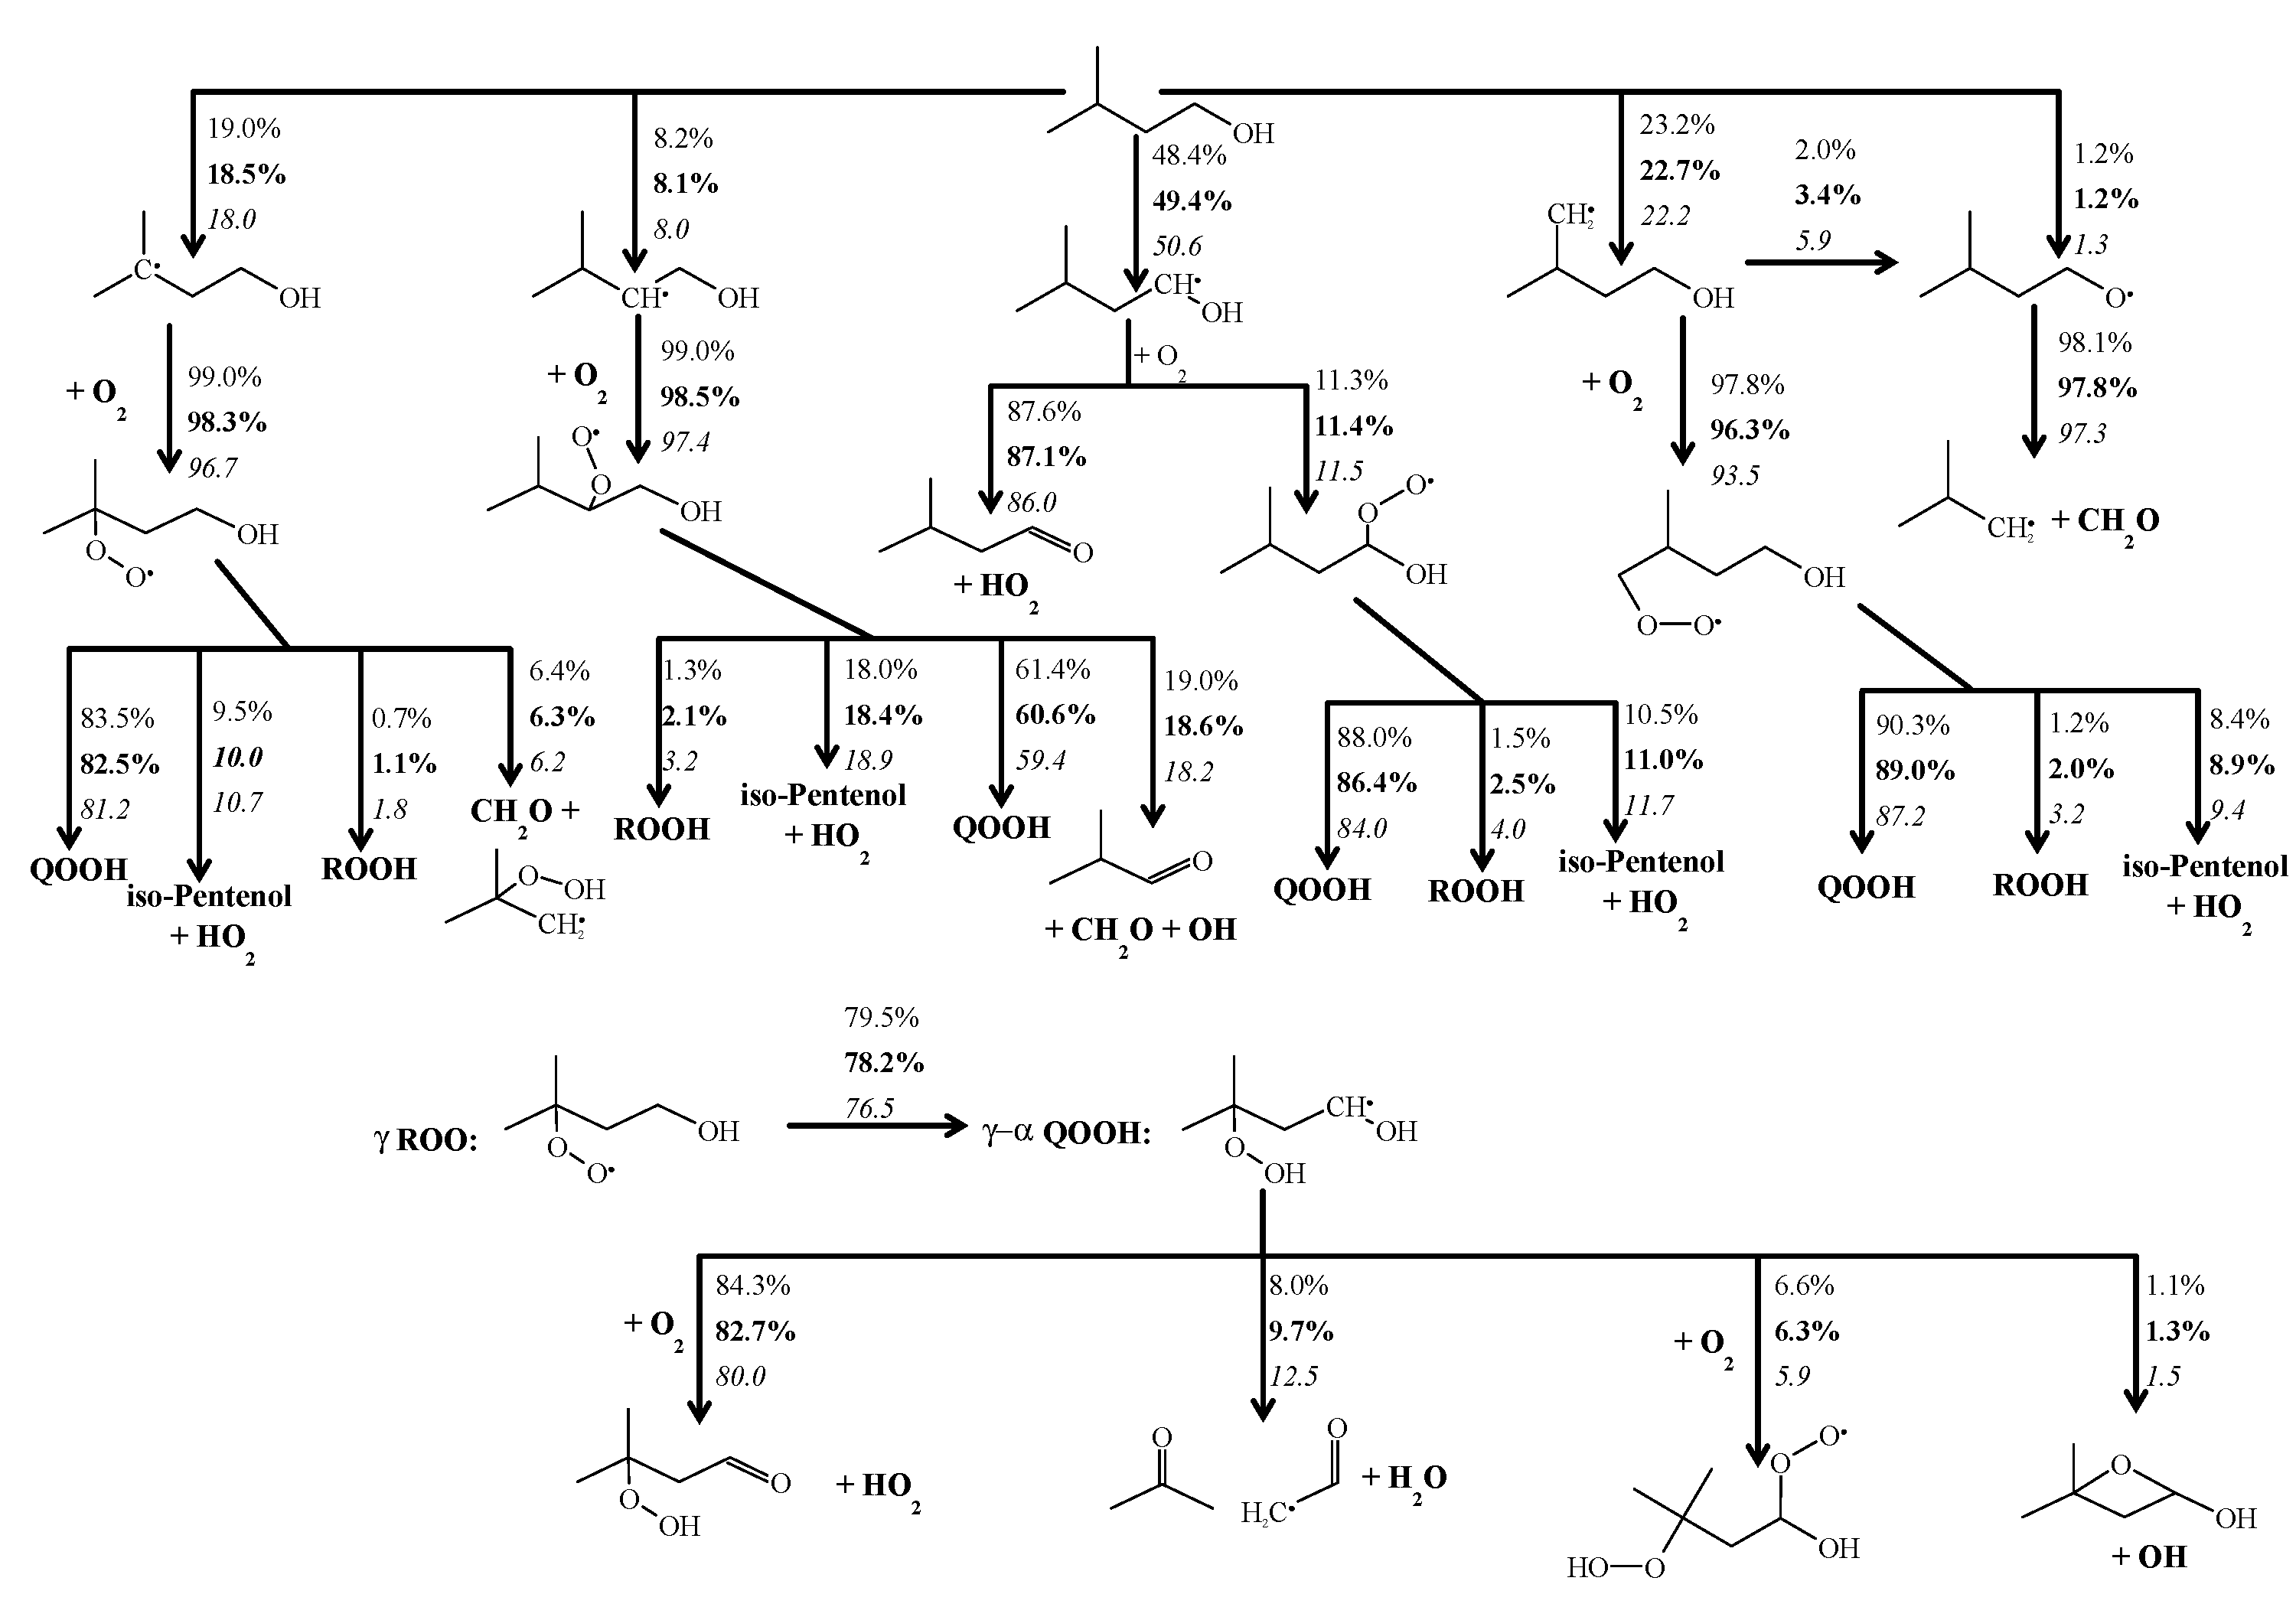
\includegraphics[width=15cm]{04-Pentanol/ipeoh-20path}
    \caption{Reaction path analysis for \iPeOH{} at \SI{800}{\kelvin},
    \SI{20}{\atmosphere}, and three equivalence ratios, based on
    constant-volume adiabatic simulations. Plain text: $\phi=0.5$.
    Bold text: $\phi=1.0$. Italic text: $\phi=2.0$. The flux is
    integrated up to \SI{20}{\percent} fuel consumption.}
    \label{fig:ipeoh-20path}
\end{figure}

\section{Conclusions}
\label{sec:ipeoh-conclusions}

New experimental ignition delay data have been collected in an RCM at
conditions of \SI{40}{\atmosphere}, $\phi=\numrange{0.5}{2.0}$, and
temperatures below \SI{800}{\kelvin}. The measured pressure histories
showed interesting behavior of slow initial pressure rise prior to a
sharp pressure rise indicating overall ignition. This pressure rise
may be attributed to the role of the Waddington mechanism in consuming
the fuel via the production and recycling of OH radicals during the
pre-ignition phase.

An existing model \cite{Tsujimura2012} for \iPeOH{} combustion has been updated with newly
calculated reaction rate coefficients and newly discovered reaction
pathways. The updated model was able to predict the ignition
delays measured in the RCM and STs fairly well, although
it was unable to reproduce the equivalence ratio sensitivity of
the low-temperature RCM ignition delay measurements. The model was
also able to qualitatively capture the slow initial pressure rise
measured during the RCM experiments, although the model was unable
to reproduce the quantitative timing of the pressure rise.

Pathway and sensitivity analyses were conducted to understand
the important reactions in the decomposition of \iPeOH{}.
The most important path for consumption of fuel radicals at low
and intermediate temperatures was the reaction of the
$\alpha$-hydroxypentyl radical with O$_2$ to form
\textit{i}-pentanal and HO$_2$ , a path that does not contribute to the
low temperature branching. However, sufficient low temperature chain
branching involving the $\gamma$ and $\delta$ fuel radicals occurred
in the model that it was able to reasonably reproduce low-temperature
ignition and reactivity observed in the experiments. Sensitivity
analysis showed that no single reaction can be modified to improve
agreement of the model with all of the conditions, and further
experimental or computational study is required to identify the
cause of the discrepancy in predictions of ignition delay
at off-stoichiometric, low-temperature conditions.
\end{document}
